%*
%* Seven Kingdoms: Ancient Adversaries
%*
%* Copyright 1997,1998 Enlight Software Ltd.
%* Copyright 2018 Timothy Rink
%*
%* This program is free software: you can redistribute it and/or modify
%* it under the terms of the GNU General Public License as published by
%* the Free Software Foundation, either version 2 of the License, or
%* (at your option) any later version.
%*
%* This program is distributed in the hope that it will be useful,
%* but WITHOUT ANY WARRANTY; without even the implied warranty of
%* MERCHANTABILITY or FITNESS FOR A PARTICULAR PURPOSE.  See the
%* GNU General Public License for more details.
%*
%* You should have received a copy of the GNU General Public License
%* along with this program.  If not, see <http://www.gnu.org/licenses/>.
%*
%*

\chapter{\textsf{BUILDINGS, WORKERS, AND LINKS}}

\section{\textsf{Constructing Your Buildings}}

\index{buildings!constructing}
\index{constructing buildings}

\begin{wrapfigure}{r}{0.1\textwidth}
    \vspace{-20pt}
    \begin{center}
        
\includegraphics[width=0.1\textwidth]{Thammer}
    \end{center}
    \vspace{-20pt}
\end{wrapfigure}

\textswab{\huge{A}} unit trained in Construction is necessary to supervise the erection of most Buildings. Although other trained units may erect certain structures, a unit trained in Construction will be able to erect them all.

To construct a Building, first select the unit that will do the construction and then \textbf{Click} on the \textbf{Build Tile}.

You will be presented with a list of structures that the unit has the ability to construct. When you \textbf{Click} on the one that you want, your cursor will change into a large black or flashing box.

\begin{wrapfigure}{r}{0.45\textwidth}
    \vspace{-20pt}
    \begin{center}
        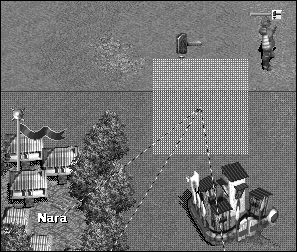
\includegraphics[width=0.45\textwidth]{Ibuildbox} % Original size.
    \end{center}
    \vspace{-20pt}
\end{wrapfigure}

The box will be black if it is over an area where you may not build. It will be flashing if it is over an acceptable area.

\textbf{Click} when the box is flashing and in the area where you want to build. Note that mines must be built atop Natural Resource deposits. 

Construction of a Building will be suspended if the building is under attack.

The speed of a building’s construction will depend on the Skill Level of the Construction worker. The higher his level, the faster the construction.

Construction workers will increase their skill whenever they are engaged in construction or repair.

If you use a Construction worker to put up a structure, he will exit the building when his work is finished. If you use a Manufacturer to build a Factory, a Miner to build a Mine, a Researcher to build a Tower of Science, or a Soldier to build a Fort, he will remain inside the building when construction has been completed.

\section{\textsf{Selling Your Buildings}}

\index{buildings!selling}
\index{selling buildings}

\begin{wrapfigure}{r}{0.4\textwidth}
    \vspace{-20pt}
    \begin{center}
        
\includegraphics[width=0.4\textwidth]{Ifullheath_building}
    \end{center}
    \vspace{-20pt}
\end{wrapfigure}

% Bold Icon?

\textswab{\huge{Y}}ou will be able to Sell your building by \textbf{Clicking} on the \$ Icon. This icon will only be visible when your structure is no more than 20\% damaged.

For the sale of an undamaged building, you will receive 50\% of the original cost of the building. If it is damaged, you will receive somewhat less, depending on the extent of the damage. You may also sell your building before you have finished its construction.

\section{\textsf{Demolishing Your Buildings}}

\index{buildings!demolishing}
\index{demolishing buildings}
    
\begin{wrapfigure}{r}{0.4\textwidth}
    \vspace{-20pt}
    \begin{center}
        
\includegraphics[width=0.4\textwidth]{Idamage}
    \end{center}
    \vspace{-20pt}
\end{wrapfigure}

% Icon here.

\textswab{\huge{I}}f your building is more than 20\% damaged, you will no longer have the option of selling it. You may either demolish it or repair it. You may demolish a building by \textbf{Clicking} on the Wrecking Ball Icon.

You will recoup no money when you demolish a building. You may also demolish your building before you have finished its construction.

% resident?

When buildings, except for Forts and Seats of Power, are demolished or sold, the workers in them will return to their Village and lose all skills that they have acquired. If there is a Construction worker in the building, he will remain a Construction worker and will be seen standing on the site of the old building. If a Fort or a Seat of Power is demolished or sold, those resident at the time will be seen standing on the site of their old building.

\section{\textsf{Repairing Your Buildings}}

\index{buildings!repairing}
\index{repairing buildings}
    
\begin{wrapfigure}{r}{0.4\textwidth}
    \vspace{-20pt}
    \begin{center}
        
\includegraphics[width=0.4\textwidth]{Irepair_building}
    \end{center}
    \vspace{-10pt} % -10pt
\end{wrapfigure}

% Bold Icon?

\textswab{\huge{A}} building may be repaired by sending a Construction unit into it. This Construction unit will not take the place of any other worker or soldier. While he is in the building, his Hammer Icon will appear next to the Sell or Demolish Icon.

Your Construction Worker will constantly repair your building, except when it is under attack. While repairing a building, he will also be increasing his skill in construction.

If you wish to take the Construction Worker out of the building, \textbf{Click} or \textbf{Right-Click} on the Hammer Icon.

\section{\textsf{Units in Buildings}}

\index{buildings!units inside}
\index{units!inside buildings}

\begin{wrapfigure}{r}{0.4\textwidth}
    \vspace{-20pt}
    \begin{center}
        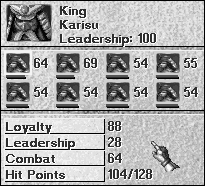
\includegraphics[width=0.4\textwidth]{Ifullfort} % Original size.
    \end{center}
    \vspace{-10pt}
\end{wrapfigure}

\textswab{\huge{W}}henever you \textbf{Click} on one of your Buildings, you will be able to see its state of repair, its color and name, all of the People currently inside and the health and status of each of them.

To see information on an individual unit inside the building, \textbf{Click} on its picture. The unit will then be highlighted in yellow, and its information will be shown below.

\subsection{\textsf{Mobilizing/Laying off Working Units}}

\index{units!laying off}
\index{units!mobilizing}

\textswab{\huge{T}}o take a worker out of his building for reassignment elsewhere, first \textbf{Click} on the building where he is working. Next, \textbf{Click} on his icon on the command bar to the right of the screen. With the unit’s icon highlighted in yellow, \textbf{Right-Click} on it. He will then exit the building with all of his skills intact.

% Outdated graphic.

\begin{wrapfigure}{r}{0.4\textwidth}
    \vspace{-20pt}
    \begin{center}
        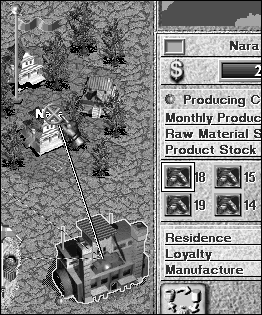
\includegraphics[width=0.4\textwidth]{Icloselink} % Original size?
    \end{center}
    \vspace{-10pt}
\end{wrapfigure}

% BUG HERE.

If you wish to lay off a worker and send him back to his Village, first select his place of work and then close the Link between it and the Village. Do this by \textbf{Clicking} inside the rotating green and yellow ring centered over the Village. With this Link closed, nobody from the Village will be able to come to work in that building. This is a good way to control your number of workers.

% Should or will?

Now select the worker by \textbf{Clicking} on his picture. He should then be highlighted in yellow. Send him back to his Village by \textbf{Right-Clicking} on the green cross (closed Link).

% X: BOLD?

You may do this in exactly the same way for your people who are working in the firms of other Kingdoms. If, in the future, you wish to hire some more workers from that Village, you will have to \textbf{Click} again on the green X, thus opening up the Link.

\subsection{\textsf{Changing a Worker’s Residence}}

\index{changing a unit's residence}
\index{units!changing residence}

\begin{center}
    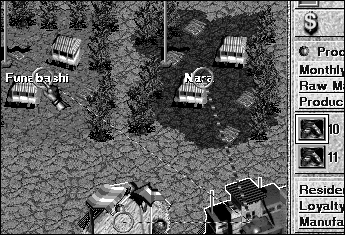
\includegraphics[width=0.6\linewidth]{Iresidencechange} % Original size.
\end{center}

\textswab{\huge{I}}f you wish to move a Worker from one Village to another, you must first \textbf{Click} on his place of work and then on his picture. If that place of work is Linked to more than one Village, you will then be able to move his residence.

% Hyphenation here.

His present Village is the one that has the double-Link line between it and his place of work. To move his residence to another Village, \textbf{Right-Click} inside the rotating ring centered on that other Village.

\section{\textsf{Linking Your Buildings}}

\index{buildings!linking}
\index{linking buildings}

\textswab{\huge{L}}inks are established when buildings are built within a certain distance of one another. You can tell if buildings or Villages are linked when there is a Linking Line connecting them.

\subsection{\textsf{Open Links}}

\index{open links}
\index{links!open}

\begin{wrapfigure}{r}{0.5\textwidth}
    \vspace{-20pt}
    \begin{center}
        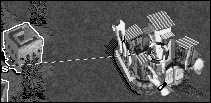
\includegraphics[width=0.5\textwidth]{Iopenlink_fort} % Original size.
    \end{center}
    \vspace{-20pt}
\end{wrapfigure}

\textswab{\huge{L}}inks are open and functioning when the yellow and green ring at the end of a line is rotating. An open Link means that goods, money, people, and influence can flow between both ends of the line.

\subsection{\textsf{Closed Links}}

\index{closed links}
\index{links!closed}

\begin{wrapfigure}{r}{0.3\textwidth}
    \vspace{-20pt}
    \begin{center}
        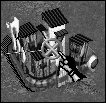
\includegraphics[width=0.3\textwidth]{Icloselink_fort} % Original size.
    \end{center}
    \vspace{-10pt}
\end{wrapfigure}

% BOLD X?

\textswab{\huge{Y}}ou may close an open Link by \textbf{Clicking} inside the rotating yellow and green ring. The ring will then change to a green X.

All flow between the two ends of the Link will then cease. This is useful for controlling the number of workers who can volunteer to work in your structures as well as for controlling the flow of goods and raw materials.

\section{\textsf{Inactive Links}}

\index{inactive links}
\index{links!inactive}

% Graphic here is different. How?

\begin{wrapfigure}{r}{0.5\textwidth}
    \vspace{-20pt}
    \begin{center}
        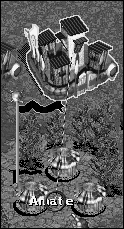
\includegraphics[width=0.3\textwidth]{Iinactivelink}
    \end{center}
    \vspace{-50pt}
\end{wrapfigure}

\textswab{\huge{L}}inks are inactive when the rings on the end of them are a solid orange in color. Inactive Links cannot be rendered active by you. They are controlled by Independent Villages or by other Kingdoms. 

\subsection{\textsf{Fort-Village Links}}

\index{fort-village links}
\index{links!fort-village}

\textswab{\huge{A}}n open Link between a Fort and a Village will allow the King or General in the Fort to exert their authority over the Village.

% Graphic here is different. BUG HERE

\begin{wrapfigure}{r}{0.5\textwidth}
    \vspace{-20pt}
    \begin{center}
        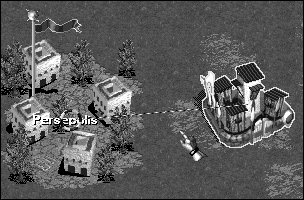
\includegraphics[width=0.7\textwidth]{Iactivelink_fort}
    \end{center}
    \vspace{-50pt}
\end{wrapfigure}

\subsection{\textsf{Village-Firm Links}}

\index{links!village-firm}
\index{village-firm links}

\begin{center}
    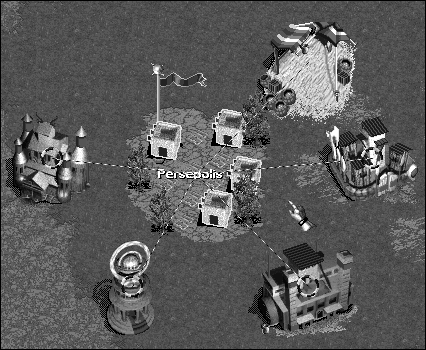
\includegraphics[width=1\linewidth]{Imultilinks} % Original size.
\end{center}

% BUG HERE.

\textswab{\huge{A}}n open Link between a Village and a Firm (any building that employs workers) will allow Peasants from the Village to volunteer to work in the Firm.

Up to eight Peasants may volunteer to fill the open working slots in each firm.

If a Firm is built outside of Linking distance to a Village, you must remember to Recruit Peasants and send them to work there. There is no way for the Peasants to volunteer.

\subsection{\textsf{Village-Market Links}}

\index{links!village-market}
\index{village-market links}

\begin{wrapfigure}{r}{0.5\textwidth}
    \vspace{-20pt}
    \begin{center}
        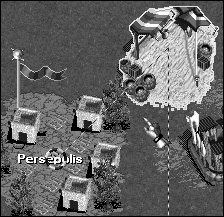
\includegraphics[width=0.5\textwidth]{Ilink_villagemarket} % Original size.
    \end{center}
    \vspace{-20pt}
\end{wrapfigure}

\textswab{\huge{A}}n open Link between a Village and a Market will allow residents of the Village to buy goods from the Market.

It is a good idea, if possible, to build a Market within Linking distance of more than one Village.

Links between your Markets and your Villages will always be open. You may not close them.

Links between Villages and Foreign Markets will be open or closed depending on whether or not the two Kingdoms have a trade treaty. You will be unable to open or close the Link manually.

\subsection{\textsf{Market-Factory Links}}

\index{links!market-factory}
\index{market-factory links}

\begin{wrapfigure}{r}{0.2\textwidth}
    \vspace{-20pt}
    \begin{center}
        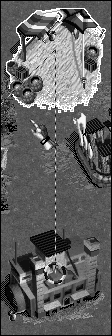
\includegraphics[width=0.2\textwidth]{Ilink_factorymarket} % Original size.
    \end{center}
    \vspace{-20pt}
\end{wrapfigure}

\textswab{\huge{A}}n open Link between a Market and a Factory will allow the Finished Goods from the Factory to be immediately sent to the Market for sale.

This will be the most efficient arrangement because it eliminates the need for a Caravan Link.

\clearpage

\subsection{\textsf{Market-Mine Links}}

\index{links!market-mine}
\index{market-mine links}

\begin{wrapfigure}{r}{0.5\textwidth}
    \vspace{-20pt}
    \begin{center}
        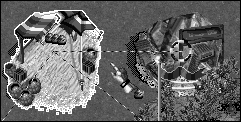
\includegraphics[width=0.5\textwidth]{Ilink_marketmine} % Original size.
    \end{center}
    \vspace{-10pt}
\end{wrapfigure}

% COMMA here

\textswab{\huge{A}}n open Link between a Market and a Mine will allow the mined Raw Materials from the Mine to be placed in the Market for sale, either to one of your Factories that is Linked to the Market or to any Caravans that call at the Market.

This arrangement is most often used when you wish to sell Raw Materials to other Kingdoms, as their Caravans will be able to call at your Markets and not at your Mines.

\subsection{\textsf{Factory-Mine Links}}

\index{factory-mine links}
\index{links!factory-mine}

\begin{wrapfigure}{r}{0.4\textwidth}
    \vspace{-20pt}
    \begin{center}
        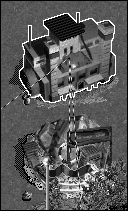
\includegraphics[width=0.4\textwidth]{Ilink_minefactory} % Original size.
    \end{center}
    \vspace{-20pt}
\end{wrapfigure}

\textswab{\huge{A}}n open Link between a Factory and a Mine will enable the Factory to receive immediate delivery of the Raw Materials that it needs to produce Finished Goods.

This arrangement is the most efficient because it eliminates the need for a Caravan to carry Raw Materials to the Factory.

\clearpage

\subsection{\textsf{Market, Factory, and Mine-Harbor Links}}

\index{links!market, factory, mine-harbor}
\index{market, factory, mine-harbor links}

\begin{center}
    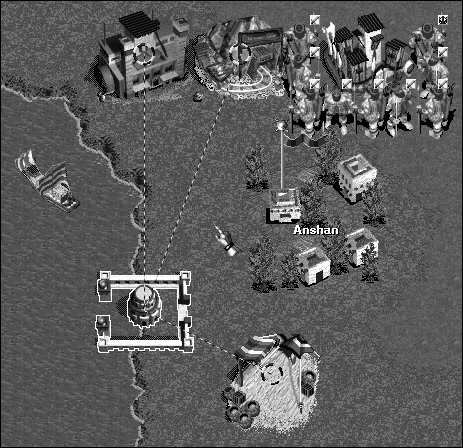
\includegraphics[width=0.95\linewidth]{Ilink_harbor} % Original size.
\end{center}

\textswab{\huge{A}}n open Link between a Market, Factory or Mine and a Harbor enable Ships calling at the Harbor to pick up either Finished Goods or Raw Materials from those places.

Your Ships will also be able to drop off their cargo from foreign lands. These goods will be immediately transferred to the Market.

The Link between your Village and your Harbor will always be open. You will not be able to close it.

A Link between your Market and a Foreign Harbor will be open or closed depending on whether or not you have a trade treaty with that Foreign Kingdom. You will be unable to open or close the Link manually.